\begin{enumerate}
\item Par lecture graphique :
\begin{enumerate}
\item Le point de la courbe d'abscisse 3 a pour ordonnée $-2$. Donc : $f(3)=-2$.

\item Le nombre dérivé $f'(3)$ est le coefficient directeur de la tangente $T$ au point d'abscisse 3.

La droite $T$ passe par le point $(3\,;\,-2)$ et, par lecture graphique, par le point $(4\,;\,2)$. 

Son coefficient directeur est donc : $\dfrac{2-(-2)}{4-3}=\dfrac{4}{1}=4$.

Ainsi : $f'(3)=4$.

\end{enumerate}

\item On considère désormais la fonction définie sur $[0\,;\,4]$ par : $f(x)=-x^3+9x^2-24x+16$.

\begin{enumerate}
\item On calcule : $f(0)=-0^3+9\times 0^2-24\times 0+16=16$.

\item Pour tout réel $x$ de l'intervalle $[0\,;\,4]$ :
\[f'(x)=-1\times3x^2+9\times x-24+0=-3x^2+18x-24.\]

\item On développe :
\[-3(x-2)(x-4)=-3(x^2-4x-2x+8)=-3(x^2-6x+8)=-3x^2+18x-24.\]
On retrouve bien l'expression de $f'(x)$ donnée.
\end{enumerate}
\end{enumerate}

\begin{enumerate}
\item[]
\begin{enumerate}[start=4]
\item On utilise la forme factorisée : $f'(x)=-3(x-2)(x-4)$.

Le facteur $x-2$ est nul en 2, le facteur $x-4$ est nul en 4.

Calculons les valeurs utiles :
\[\text{On a déjà : } f(0)=16,\]
\[f(2)=-2^3+9\times 2^2-24\times 2+16=-8+36-48+16=-4,\]
\[f(4)=-4^3+9\times 4^2-24\times 4+16=-64+144-96+16=0.\]

On obtient :

\begin{center}
\begin{tikzpicture}
\tkzTabInit[lgt=2.8,espcl=2.8]{$x$/1,$-3$/1,$x-2$/1,$x-4$/1,$f'(x)$/1,$f(x)$/2}{$0$,$2$,$4$}
\tkzTabLine{,-,t,-,t}
\tkzTabLine{,-,z,+,t}
\tkzTabLine{,-,t,-,z}
\tkzTabLine{,-,z,+,z}
\tkzTabVar{+/$16$,-/$-4$,+/$0$}
\end{tikzpicture}
\end{center}

\item D'après le tableau de variation, le minimum de la fonction $f$ sur l'intervalle $[0\,;\,4]$ est $y=-4$, il est atteint pour $x=2$.

\end{enumerate}
\end{enumerate}
